\section{Introduction}

Ideally we would like mechanistic interpretability to provide guarantees
about the computational process used by a model. We would like features
to be
\begin{enumerate}
	\item causal
	\item composable
	\item closed-form
\end{enumerate}
However most existing techniques, such as sparse autoencoders (SAEs),
produce features that can perform arbitrarily badly on these desiderata.
Feature splitting breaks compositionality. They can't usually be
statically analyzed (though bilinear SAE variants can be). Sparsity
trades off against reconstruction fidelity, limiting the extent to which
features can be used for steering.

Arguably the simplest interpretability technique is a linear probe, and
the simplest control technique is a steering vector. They are remarkably
robust compared to unsupervised techniques such as SAEs, but require
labeled contrastive datasets. We propose a MoEfication technique based
on decomposing a representation space into a set of contrastive
classifiers. Each
classification corresponds to a representative vector. Inputs are
encoded as a series of classifier outputs, and reconstructed from a
weighted average of the representative vectors. This has several
advantages over SAEs:
\begin{enumerate}
	\item It effectively gives steering for free.
	\item Outputs are bounded.
	\item The representative vectors admit static interpretation in
	principle; making that real is currently an open problem
	(Section~\ref{sec:prelim-autointerp}).
	\item Feature space is structured.
\end{enumerate}
The measured version of this pitch is Figure~\ref{fig:teaser}; the
full evaluation, including where it cuts against the proposal, is
Section~\ref{sec:prelim}.

\begin{figure}[tp]\centering
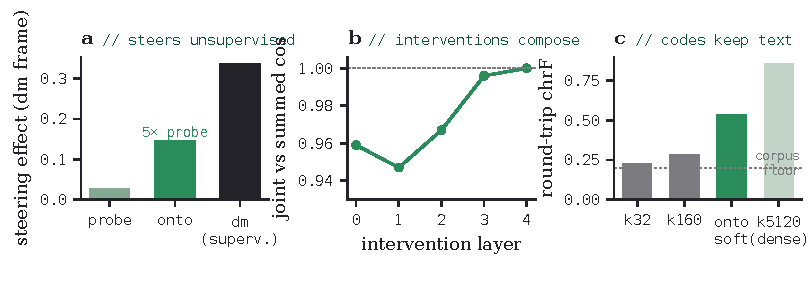
\includegraphics[width=\linewidth]{figures/fig-teaser.pdf}
\caption{The proposition, measured. Left: forcing classifications
moves decodes along the supervised difference-of-means direction
$0.43\times$ as far as supervised steering itself and $5\times$
further than probe directions, the strongest unsupervised arm tested
(Table~\ref{tab:steer-overlay}). Center: joint interventions point
where the summed single interventions point, exactly so in the final
layer (working notes). Right: the sparse SAE tier's codes lose most
text before any intervention is applied (round-trip chrF
$0.23$--$0.29$ against a $0.20$ corpus floor) while the Ontologizer's
soft code preserves it, so low-collateral steering is available only
to the soft architectures; the dense k5120 SAE preserves text but is
not a sparse steering code (working notes).}
\label{fig:teaser}
\end{figure}

\section{Assumptions}

This proposal assumes:
\begin{itemize}
	\item \textbf{Steering is inherent to the training objective.}
	The dictionary vectors must also be high quality steering vectors;
	interpretability and steering are treated as the same problem.
	\item \textbf{Weights are themselves interpretable} (for certain architectural choices).
	\item \textbf{Clustering rather than decomposition.} Representations
	are grouped into mutually contrastive categories rather than
	decomposed into independently firing features. The clustering framing
	is counterintuitive unless you arrive at it from Leiden-style
	community detection.
	\item \textbf{Categorical structure is imposed on features.}
	\item \textbf{Interpretability gets a cheap forward pass.}
	\item \textbf{Concepts compose linearly.} Concepts must be additive to be
	useful.
	\item \textbf{Dictionary learning is all you need}, in a nonstandard
	form: the dictionary forms a basis for the representation rather than
	a target.
	\item \textbf{Representations are not themselves quantized.} The
	learned dictionary serves as a basis for the representation rather
	than a discrete codebook; quantization comes from sharpening of
	classifications over that basis.
	\item \textbf{Interpreting a well trained model is the same problem
	as interpreting the data and training tasks.}
\end{itemize}

\subsection{Pivotal assumptions}
Two of these are pivotal: some version of the linear representation
hypothesis is true, and latent space is in some way ``natural''.

\subsection{Concerns}

\paragraph{Timelines could be too short}
We'll just have to go faster.

\paragraph{Contrastive classifiers might not be expressive enough}
This is what the reconstruction benchmarks are for. The preliminary
numbers (Section~\ref{sec:prelim}) put a price on the constraint; the
open question is whether steering quality justifies it.

\paragraph{Steering could push it too far off manifold}
This is an open problem in mechinterp. Diffusion steering is one
candidate to address it\cite{wagenmaker2025}.
If we can't solve the problem it still gives good data to test steering
methods. e.g.\ can we RL a model for high/low scores on a classification
and have it converge faster than paired steering or PCA vectors?
A first pass exists: a REINFORCE policy over steering directions on
frozen \texttt{resid\_nc\_hm}, rewarded by one classification's
quantile-normalized score at a matched intervention budget, converges
cleanly in the differentiable in-embedding tier, saturating within
roughly 40 steps at flat collateral (Figure~\ref{fig:rl}). Neither the
decode-cycle tier nor the convergence race against paired steering has
been run; the race is the test this paragraph proposes.

\begin{figure}[tp]\centering
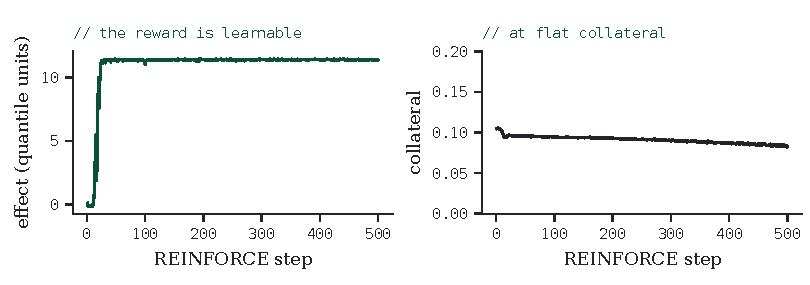
\includegraphics[width=\linewidth]{figures/fig-rl.pdf}
\caption{REINFORCE against a single frozen classification's
quantile-normalized score, in-embedding tier. The policy saturates the
reward within roughly 40 steps while collateral stays at its starting
level; a classification is a trainable objective.}
\label{fig:rl}
\end{figure}

\paragraph{Representations could be too soft/dense/high entropy}
This is highly correlated across all feature-based interp (SAEs,
transcoders, J-space). Dividing representations across orthogonal
categorical subspaces makes it possible to interpret the conceptual
basis vectors even if the representations are dense mixtures.

\paragraph{Ontofeatures could be too polysemantic}
Orthogonality \& categorical constraints give a theoretical inductive
bias to monosemanticity. As long as they have decent explanatory power
we can do eigendecomposition; polysemanticity decreases with parameter
count and we have more directions to increase parameters (in addition to
increasing width we can increase head size or stack more layers).
A first star sweep tests the scaling prediction at reduced training
(architecture and terms defined in Section~\ref{sec:arch}): seven
configurations around the shared $h{=}32$, $k{=}32$, $l{=}5$ shape,
varying one axis at a time, each trained 4 epochs (62k steps; the
retrain recipe's 24 epochs is 372k steps). No measured axis delivers
the predicted rise: head coherence shows no positive relation to
parameter count
(Spearman $+0.14$ for mean $z_{\cos}$, $-0.54$ for the fraction above
$z{=}2$), usage imbalance grows with size ($+0.86$), and the cleanest
per-axis trend runs opposite to the claim, coherence falling
monotonically as entries per head grow ($k{=}16/32/64$: mean $z_{\cos}$
$20.2/6.3/3.7$). One confound is recorded: the widest model ($h{=}64$)
has not converged at this budget (tail MSE $20\times$ the others), so
its collapse is not evidence (Figure~\ref{fig:scaling}). Seven points
at short training are weak evidence either way; full-length retrains
are the missing control.

\begin{figure}[tp]\centering
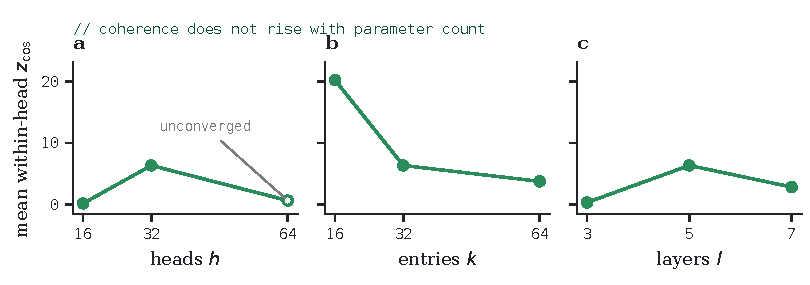
\includegraphics[width=\linewidth]{figures/fig-scaling.pdf}
\caption{Head coherence against each parameter axis of the star sweep,
all runs at 4 epochs (62k steps) of the retrain recipe's 24. No axis
delivers the predicted rise; the entries axis falls monotonically. The
open marker is the unconverged $h{=}64$ run.}
\label{fig:scaling}
\end{figure}

\paragraph{Interpreting ontofeatures could be otherwise intractable}
This would imply the universality hypothesis is false and is highly
correlated with intractability of other interpretability agendas.
Submodules could be interpretable even if features aren't.

\paragraph{Training could be intractable}
Sparsity trades against sample/compute efficiency; preliminary
experiments suggest we have less need for a sparsity constraint
(working notes).

\paragraph{Too many hyperparameters/too hyperparameter dependent}
This generally becomes less of an issue with scaling; preliminary
experiments show most changes to hyperparameters just change the rate of
convergence (working notes).

\paragraph{Doesn't converge in the limit}
Collapse in one layer would propagate down the stack. Candidate causes:
underparameterization, a really bad optimizer, bad initialization, a bad
loss term.

\paragraph{Not orthogonal in the limit}
$\mathrm{cossim}_h$ (Section~\ref{sec:loss}) penalises overlap between
heads but does not
guarantee disjoint support at convergence. The head geometry
(Figure~\ref{fig:head-simplex}) is built to make orthogonality the cheap
solution, not to force it.

\paragraph{Might not generalize out of distribution}
The same concern applies to every feature-based technique. Closed-form
interpretation of the dictionary is the mitigation: a statically
interpreted basis does not depend on the input distribution, though the
classifications over it do.

\paragraph{Inference too expensive}
Each layer adds $h \cdot k$ classifications per sample
(Section~\ref{sec:arch}), with $k$ small;
the code is computed without materializing a wide feature space. The
cost is the extra decoder passes for deep supervision during training.

\paragraph{Autointerp doesn't work on parameters/eigenfeatures}
In the preliminary experiments, parameter-space decodes of feature
directions failed as descriptions outright
(Section~\ref{sec:prelim-autointerp}). This is direct evidence against
the static-interpretability claim.
